\documentclass[a4paper]{article}
\usepackage{color}
\definecolor{grey}{rgb}{0.95,0.95,0.95}
\definecolor{keyword}{rgb}{0,0,0.95}
\definecolor{comment}{rgb}{0.95,0,0}
\definecolor{string}{rgb}{0,0.65,00.65}

\usepackage{listings}
\lstset{backgroundcolor=\color{grey},
        language=C, 
        numbers=left,
        numbersep=6pt,
        basicstyle=\small\ttfamily,
        extendedchars=true,
        tabsize=3,
        keywordstyle=\color{keyword}\bfseries,
        commentstyle=\color{comment},
        stringstyle=\color{string}\itshape,
        columns=fullflexible,
        keepspaces=true,
}
\usepackage{fullpage,graphicx,url}
\begin{document}
\begin{center}
{\bf\Large Buildroot for cross-compiling GNU Radio to embedded boards}\\
\today
\end{center}
The Raspberry Pi\{3,4\} (RPi) is a single board computer designed -- for the characteristics
we are interested in for Software Defined Radio applications -- around a 
quad-core ARM processor clocked at 1.5~GHz with 1, 2 or 4~GB random access memory.
The operating system is stored on a microSD card and is hence easily updated
from the host computer (never {\em ever} compile on the target embedded board). Generating
a dedicated toolchain -- as opposed to using a readily available binary distribution --
allows for optimizing instructions for the chipset available on the targeted platform.

Our objective is to {\bf execute GNU Radio on the RPi} in order to run some
pre-processing on the embedded board before sending the processing result to
the PC (e.g. receiving a broadcast FM station on the RPi and send the audio
output to the PC through a Zero-MQ link).

\section{Buildroot for RPi}

Buildroot is a framework providing a consistent set of
\begin{itemize}
\item cross-compilation toolchain for the host (usually Intel x86/AMD64 processor)
\item libraries and userspace applications for the ARM target,
\item Linux kernel for the target,
\item bootloader for embedded target board initialization in order to load the Linux
kernel in charge of supervizing userspace applications.
\end{itemize}

This consistency avoids many pitfalls when cross-compiling target applications 
or kernel modules on the host. Obviously the low-computational power target is 
{\em not} designed for intensive computational load such as compiling GNU Radio, and
{\tt gcc} should actually not even be available on the target, neither is the SD
card with its finite number of write cycles designed for large compilation (at least
make {\tt /tmp/} a RAM filesystem if trying such a compiltion on the target).

Installing the result of Buildroot cross-compilation on the Raspberry Pi4 is 
described at \url{https://github.com/buildroot/buildroot/tree/master/board/raspberrypi} but
the documentation on this web page is not up to date (?!):
\begin{enumerate}
\item {\tt git clone https://git.busybox.net/buildroot}
\item {\tt cd buildroot}
\item {\tt make raspberrypi4\_64\_defconfig}
\end{enumerate}
fetches the Buildroot archive, and configures for the Redpitaya4 in 64~bit mode (obviously
for RPi3, select {\tt raspberrypi3\_64\_defconfig}).
Because Python support for GNU Radio will require the {\tt glibc} library rather than the default
{\tt uClibc}, we must tune the default configuration
\begin{enumerate}
\setcounter{enumi}{3}
\item {\tt make menuconfig}
\item Toolchain $\rightarrow$ C library (uClibc-ng) $\rightarrow$ glibc
\item Exit
\end{enumerate}

Once the proper C-library has been selected
\begin{enumerate}
\setcounter{enumi}{6}
\item {\tt make}
\end{enumerate}
builds all tools
needed for cross-compilation. This operation will take about 40~min on an 8-core 2.33~GHz Xeon 
CPU with fast internet connexion and require 7.4~GB of hard disk space. While compiling, 
Buildroot {\em only updates files stored} in the 
{\tt output} directory. Thus, removing this directory (and sub-directories) will return to
the original Buildroot configuration. All software related to the host computer -- Intel x86/AMD64
architecture most of the time -- is located in {\tt output/host}, while all software related
to the target (here ARM architecture) is stored in {\tt output/target}. We shall not be
interested in the content of the directory in which source files are stored but might have
to erase some of its content to force re-compilation: such files are stored in the {\tt output/build}
directory. Finally, the last compilation stage will result in a complete image including bootloader,
kernel, libraries and userspace applications: this file is stored in {\tt output/images}.

After completing buildroot compilation, we find in the {\tt output/images} directory 
the file {\tt sdcard.img} which 
holds the binary datastream (about 150~MB) to be stored on the microSD card holding the 
operating system to 
be run on the RPi. Here, ``stored'' doe not mean copying since we must clone each byte from 
the binary file to the storage medium. Such an operation is achieved under GNU/Linux with the
Disk Dump {\tt dd} command.


\includegraphics[width=.7cm]{danger} 
The following line might definitely {\bf corrupt a hard disk} if the wrong storage
medium is selected. Alway {\bf check} the name of the peripheral associated with
the SD card (\verb~dmesg | tail~) before running the {\tt dd} command.

The image resulting from Buildroot compilation is transfered to the microSD card with\\
\colorbox{white}{\begin{minipage}{0.9\textwidth}
sudo dd if=output/images/sdcard.img of=/dev/sdc
\end{minipage}} 
where we have on purpose selected the {\tt /dev/sdc} peripheral name in this example
since it is ever hardly used. Usually, the microSD card is accessed as {\tt /dev/sdb} 
(second hard disk storage medium compatible with the Linux SCSI driver)
or {\tt /dev/mmcblk0} (internal SD medium interface).

In case a Desktop Manager or a File Manager is used, make sure the SD card is unmounted
before executing {\tt dd}, as these tools will interfere with the cloning process.

\noindent\fbox{\parbox{\linewidth}{

\includegraphics[width=.7cm]{danger} %\danger 
{\bf Warning}: the content of the SD card, or any storage medium associated with
the last argument of this command, will be {\bf definitely} lost. Make sure, double check,
the name of the peripheral on which the Buildroot image will be stored.}}

Once the image has been flashed on the SD card, we can see two partitions: the first one
is a VFAT (format compatible with Microsoft Windows) with the devicetree, the Linux 
kernel and the bootloader, and a second one holding the GNU/Linux userspace filesystem
({\tt rootfs}).

\section{Adding custom packages (GNU Radio and PlutoSDR/UHD}

So far we have compiled a standard Buildroot image without dedicated GNU Radio support.
Dedicated packages not selected in the default configuration can be activated. This is 
achieved from the Buildroot directory with {\tt make menuconfig} and selecting {\tt Target 
packages}. Searching (``/'' command as in {\tt vi}) allows for quickly finding the appropriate
package, such as GNU Radio. 

So far we have only worked with ``official'' Buildroot packages properly maintained by
the Buildroot community. Some packages are not yet integrated in the official repository
but can nevertheless be appended as external packages thanks to the {\tt BR2\_EXTERNAL}
mechanism. As an example of supporting the PlutoSDR thanks to {\tt gr-iio}, this support
is available thanks to the {\tt BR2\_EXTERNAL} repository found at 
\url{https://github.com/oscimp/PlutoSDR} and most significantly its {\tt for\_next} branch.
Hence, after going to a any directory out of the Buildroot source tree:
\begin{enumerate}
\item \verb~git clone https://github.com/oscimp/PlutoSDR~
\item \verb~cd PlutoSDR~
\item \verb~git checkout for_next~
\item \verb~source sourceme.ggm~
\end{enumerate}

Now that the {\tt BR2\_EXTERNAL} has been cloned, the appropriate branch selected, and the
environment variables set (last command), return in the Buildroot directory and
{\tt make menuconfig}. Running {\tt make menuconfig} will now show a new menu named 
{\tt External options} including
{\tt gr-iio}, {\tt libuhd} or {\tt gnss-sdr}. 

\begin{enumerate}
\item \verb~make menuconfig~
\item \verb~/eudev~
\item Select the last item indicating {\tt BR2\_ROOTFS\_DEVICE\_CREATION\_DYNAMIC\_EUDEV} and
replace {\tt /dev management} with {\tt Dynamic using devtmpfs + eudev}
\item \verb~/python3~
\item Select item (4) indicating {\tt BR2\_PACKAGE\_PYTHON3}
\item \verb~/gnuradio~
\item Select item (1) indicating {\tt BR2\_PACKAGE\_GNURADIO}
\item Select additional GNU Radio functionalities as needed (we will need {\tt gr-zeromq support}
and {\tt python support})
\item \verb~/osmosdr~
\item Select {\tt BR2\_PACKAGE\_GR\_OSMOSDR} (with Python support and Osmocom RTLSDR support)
\item in {\tt External options} select {\tt uhd} and for the B210 {\tt b200 support} and 
{\tt python API support}, 
\item in {\tt External options} select {\tt gr-iio} for PlutoSDR support.
\end{enumerate}

The resulting file will be about 550~MB, requiring increasing the configuration in {\tt .config}
with {\tt BR2\_TARGET\_ROOTFS\_EXT2\_SIZE="420M"}.

\section{GNU Radio on RPi}

As a demonstration of the proper operation of GNU Radio on the embedded board, we
generate using GNU Radio Companion a command line interface (``No GUI'') processing flow 
since obviously no graphical interface is running on the embedded target, and will execute 
the resulting Python3 script on the Raspberry Pi4. The audio stream resulting from broadcast
FM demodulation will be streamed to the host PC for playing on the sound card.

On the host computer, run GNU Radio Companion (as part of GNU Radio 3.8) and generate
the following chart:

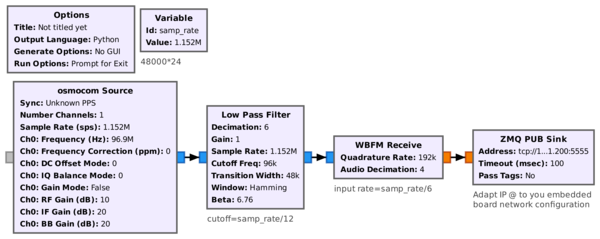
\includegraphics[width=\linewidth]{target}

The generated Python script will be transfered and run on the RPi platform. Make sure
to adapt the 0-MQ TCP IP address to the RPi address: the server is running on the local board
and being a Publish-Subscribe (like UDP broadcast) configuration, any client connecting to
the server running on the local board will be streamed the dataflow. The IP address must
match the subnet of the host PC for easier routing configuration and the port might be
anything above 1024. The only constraints on this flowgraph is to achieve a final sampling
rate matching the PC sound card sampling rate (here 48~kHz) following an integer decimation,
here tuned with a sampling rate of $48\time 24$~kS/s. The first low-pass filter selects
a unique FM broadcast station while still keeping enough bandwidth ($\geq$200~kHz) for
wideband FM demodulation, and the FM demodulator add the second decimation stage.

\section{Communication RPi to PC}

After processing the raw RF (I/Q) signal collected from the FM broadcast band on the RPi, 
and preprocessing FM demodulation on the embedded target board, the audio stream is
sent PC over 0-MQ.

\begin{center}
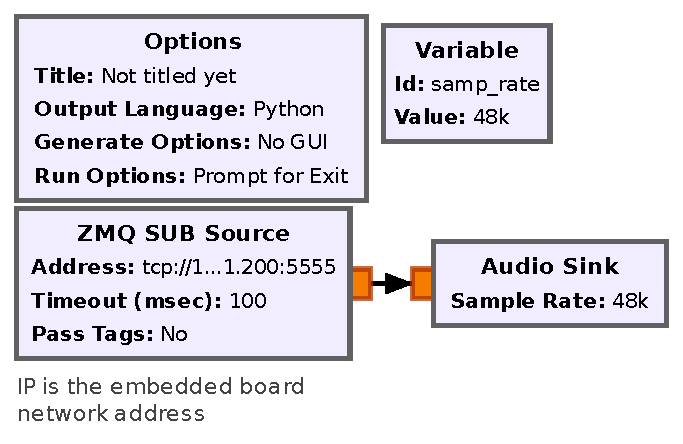
\includegraphics[width=.59\linewidth]{host}
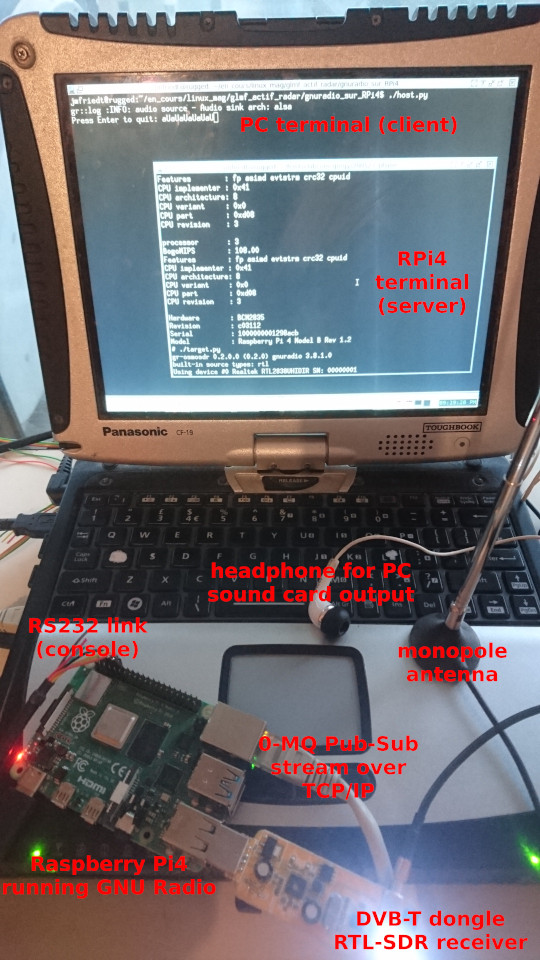
\includegraphics[width=.39\linewidth]{IMG_20200527_211928small.jpg}
}
\footnotesize{Left: client flowchart, fetching a 0-MQ subscribe datastream and feeding
the sound card of the host PC. Right: experimental testbed, with the RPi4 connected
though virtual serial port and Ethernet to the laptop PC. The RPi4 collects an I/Q stream
from the DVB-T dongle tuned to an FM-broadcast station, streams the demodulated audio
flow to the PC, allowing to listen to the program on the headset connected to the sound card
output. Not heard on this figure is the excellent sound quality heard on the headset, demonstrating
perfect functional capability of this setup.}
\end{center}

\section{Software development}

We are interested in tuning the {\tt gnss-sdr} functionalities. The source code of
the software has been downloaded in the {\tt output/build} directory. The build directory 
for the target system is found in {\tt output/build/gnss-sdr-0.0.12/buildroot-build/} while
a separate {\tt output/build/gnss-sdr-0.0.12/build} allows for simultaneously testing source
code modifications on the host PC. The output of compiling ({\tt make}), either in 
{\tt buildroot-build} (ARM target) or {\tt build} (x86 target), is found in {\tt 
src/main/gnss-sdr}.
\end{document}
